%-----------------------
% Title page
%-----------------------
\begin{titlepage}
  \centering

  \textsc{ELEC4630 Assignment 2}\\
  \vspace{9cm}

  \rule{\linewidth}{0.5pt}\\

  \vspace{1em}
  \LARGE\textsc{Question 1}\\
  \vspace{1em}

  \LARGE\uppercase{\textbf{{Medical Image Segmentation}}}\\

  \rule{\linewidth}{2pt}\\

  \vfill

  \normalsize{Deren Teo (4528554)}
  \vspace{1cm}

\end{titlepage}

%-----------------------
% Report body
%-----------------------
\section{Introduction}

Segmentation of medical images is of key importance to identifying and characterising features relevant to medical diagnoses \cite{dinesh_2013}. Segmentation is traditionally performed manually by radiologists and other specialists; however, manual segmentation is becoming increasingly impractical due to the vast and increasing quantity and variety of medical images requiring examination \cite{dinesh_2013}. As a result, accurate automated algorithms are of interest to alleviate the burden on medical professionals \cite{dinesh_2013}. This report presents two simple algorithms for the segmentation of the inner and outer walls of the left ventricle in cardiac MRI images. The first approach relies solely on morphology and contours, while the second approach applies the Viterbi algorithm to the segmentation problem. The application of the algorithms to a sequence of images can assist cardiologists in diagnosing the efficacy of a beating heart \cite{elec4630_2023}.

\section{Background Theory}

There is abundant literature on medical image segmentation, much of which exceeds the scope of this report. However, knowledge of successful methods is nonetheless useful in the design of simpler solutions to a similar task. This section covers active contours and the Viterbi algorithm for image segmentation, skipping for sake of brevity other techniques such as fast marching, level sets, and globally minimal surfaces. The section concludes with a short description of the important anatomical features present in the provided sequence of cardiac MRI images and relevant to the ventricle segmentation task.

\subsection{Active Contours}

An active contour, or ``snake" as introduced by Kass et al. \cite{kass_1988}, is a 2D curve with the property of being adaptable to features such as edges and lines in an image \cite{biswas_2007}. The snake iteratively conforms to features in the image by means of an energy minimisation process \cite{biswas_2007}. The image must therefore have an associated energy map pre-defined by the algorithm designer. For example, Kass et al. \cite{kass_1988} suggest a weighted set of features based on lines, edges, and line terminations \cite{biswas_2007}.

The formulation of the internal energy state of a snake can be understood as the weighted sum of two terms: membrane energy, and thin-plate energy \cite{biswas_2007}.

\begin{align}
  E_{int}(\nu_i) = \alpha_i \underbrace{| \nu_i - \nu_{i-1}|^2}_{\text{membrane term}} +
                   \beta_i \underbrace{| \nu_{i+1} - 2\nu_i + \nu_{i-1}|^2}_{\text{thin-plate term}}
\end{align}

The above equation, from \cite{biswas_2007}, calculates the internal energy of control point $i$ of snake $\nu$.

The membrane term evaluates to the square of the distance between successive control points, and is therefore minimised by equidistant and collinear points \cite{biswas_2007}. As a result, the minimum internal energy of an open snake is achieved by a linear configuration, with equally spaced control points \cite{biswas_2007}. The membrane term may intuitively be considered to provide ``elasticity'' to the snake, causing it to shrink to fit a minimum energy state \cite{biswas_2007}.

Conversely, the thin-plate term intuitively provides a ``stiffness'' which enforces smooth curves in a minimum energy state, rather than sharp bends in the snake \cite{biswas_2007}. The minimum internal energy of a closed snake is therefore achieved by a circular shape, which will eventually collapse into a point due to the elasticity term under no external energy influence \cite{biswas_2007}.

The combination of these two terms allows the snake to fit a smooth contour to features in an image, and has been demonstrated for medical image segmentation. For example, Bamford \cite{bamford_1999} (from \cite{biswas_2007}) demonstrates the segmentation of a cell nucleus using a closed snake.

\begin{figure}[ht]
  \centering
  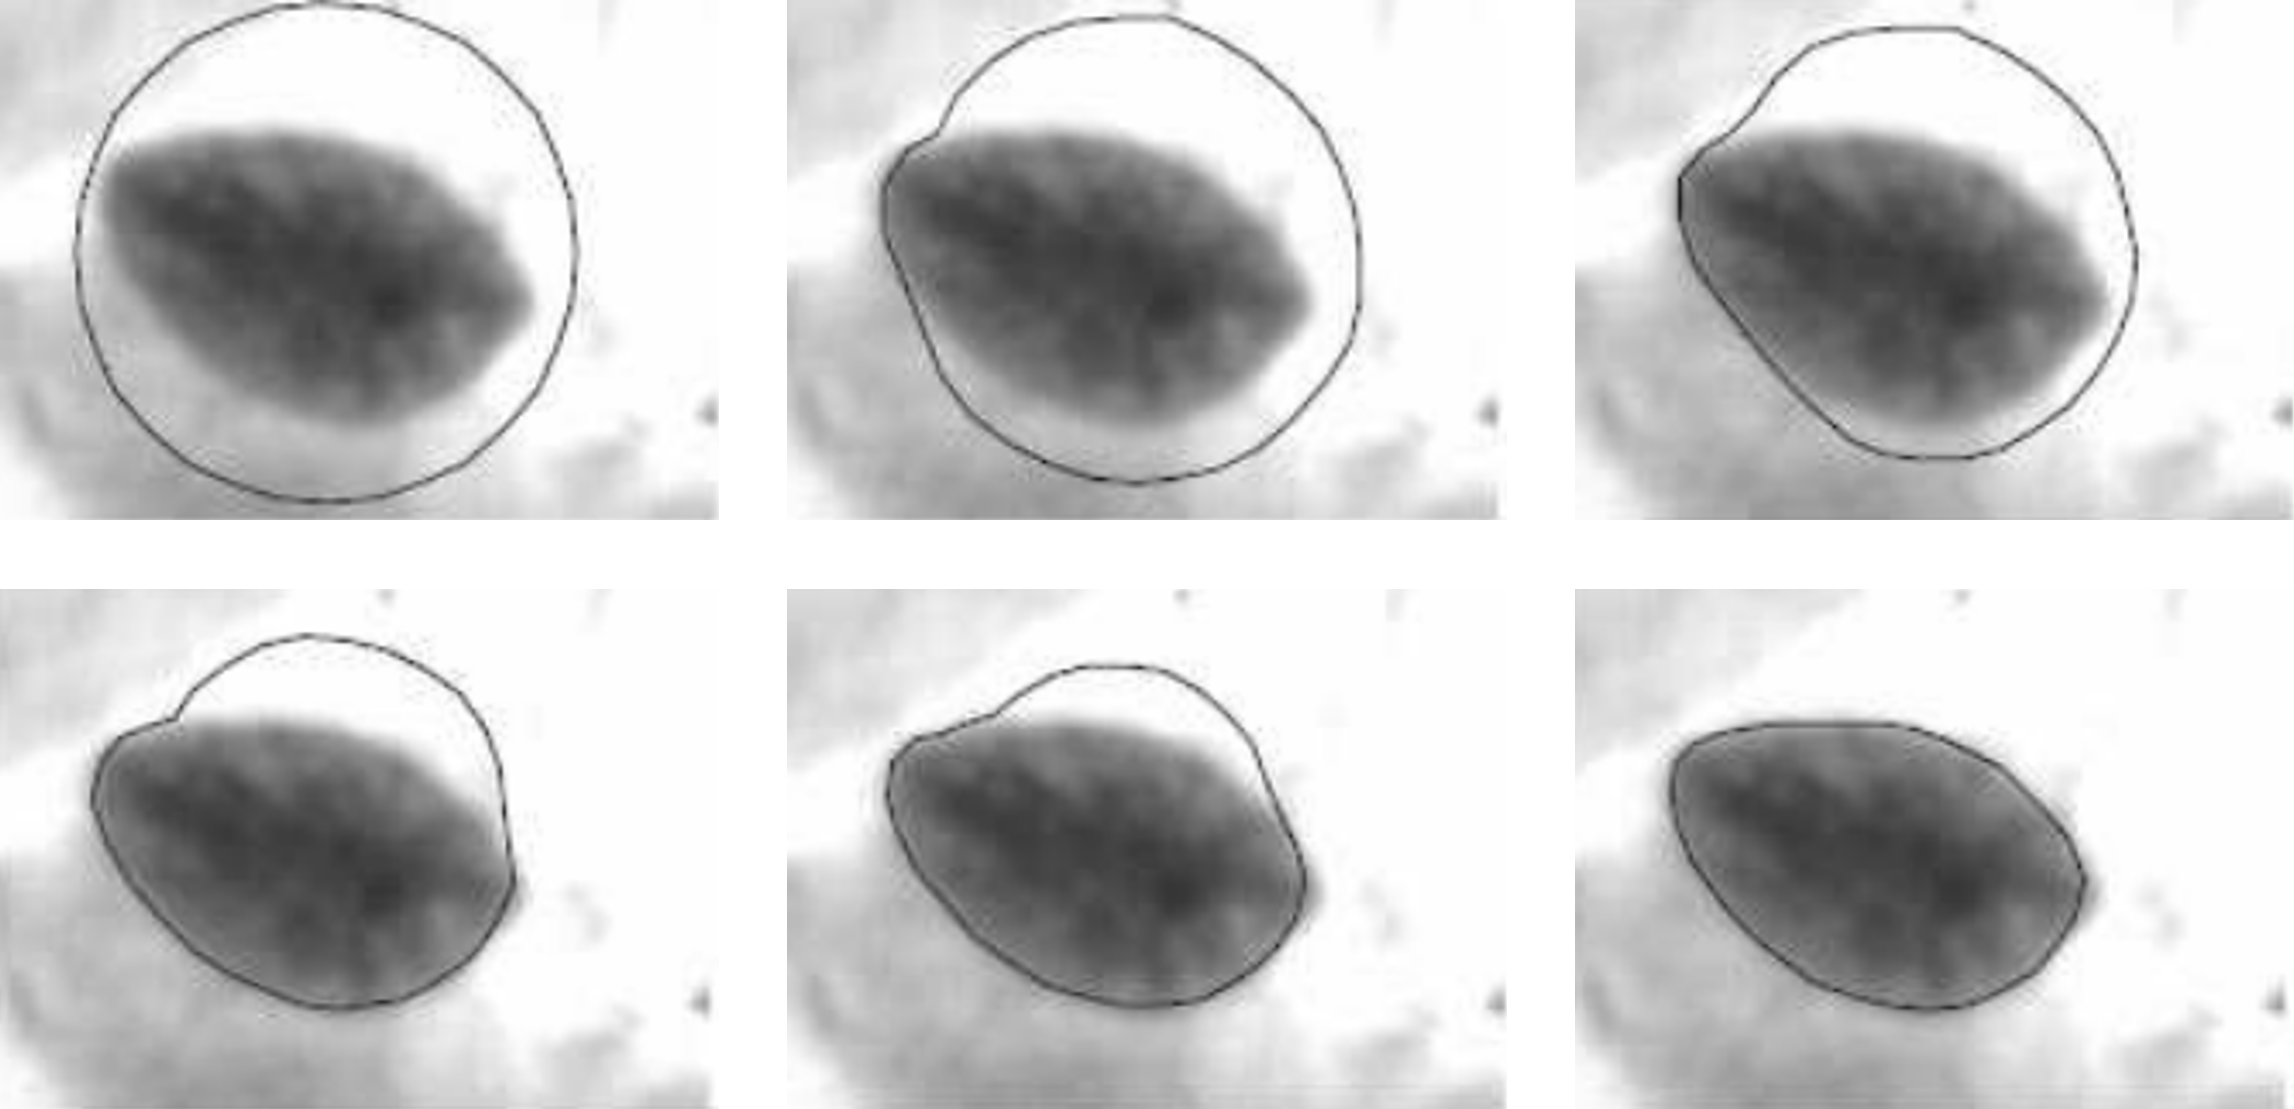
\includegraphics[width=0.9\textwidth]{images/q1_snakes.png}
  \caption{Segmentation of a cell nucleus using a closed snake (from \cite{bamford_1999}, presented in \cite{biswas_2007}).}
\end{figure}

\subsection{Viterbi Algorithm}

By contrast, the Viterbi algorithm leverages dynamic programming to optimise the fit of a contour to an image by evaluating a large set of possible solutions and selecting the minimum cost solution \cite{biswas_2007}. The Viterbi algorithm is conceptually similar to Dijkstra's algorithm, but calculates the lowest cost path through a \textit{trellis} rather than a network \cite{biswas_2007}.

To apply the Viterbi algorithm to the search space of a closed snake, the circular domain of the snake can be unwrapped into a linear trellis \cite{biswas_2007}. An example of this is provided by Figure \ref{fig:trellis}.

\begin{figure}[ht]
  \centering
  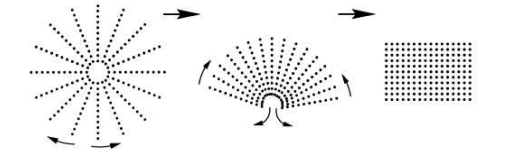
\includegraphics[width=0.7\textwidth]{images/q1_trellis.png}
  \caption{A closed snake search space unwrapped into a trellis (from \cite{biswas_2007}).}
  \label{fig:trellis}
\end{figure}

One can then apply the concept of a Hidden Markov Model (HMM) to calculate a ``most-probable'' path through the trellis, representing a closed snake, given a set of observations and probabilities. The Viterbi algorithm defines three sets of probabilities: initial, transition and emittance. Arbitrarily starting at the left side of the trellis, the initial probabilities define the likelihood of the snake passing through each point in first column of the trellis, given no previous information about the problem. The transition probabilities define the likelihood of transitioning from one state to another between columns of the trellis. Finally, the emittance probabilities define the likelihood of the snake passing through certain points in the trellis given a set of observations; hence, the segmentation problem can be formulated as the determination of a hidden true state of a snake, given observations from an image.

\subsection{Cardiac MRI Anatomy}

Finally, a short description is warranted to elucidate key anatomical features in the provided sequence of cardiac MRI images. Figure \ref{fig:cardiac_anatomy} annotates the first image in the sequence.

\begin{figure}[ht]
  \centering
  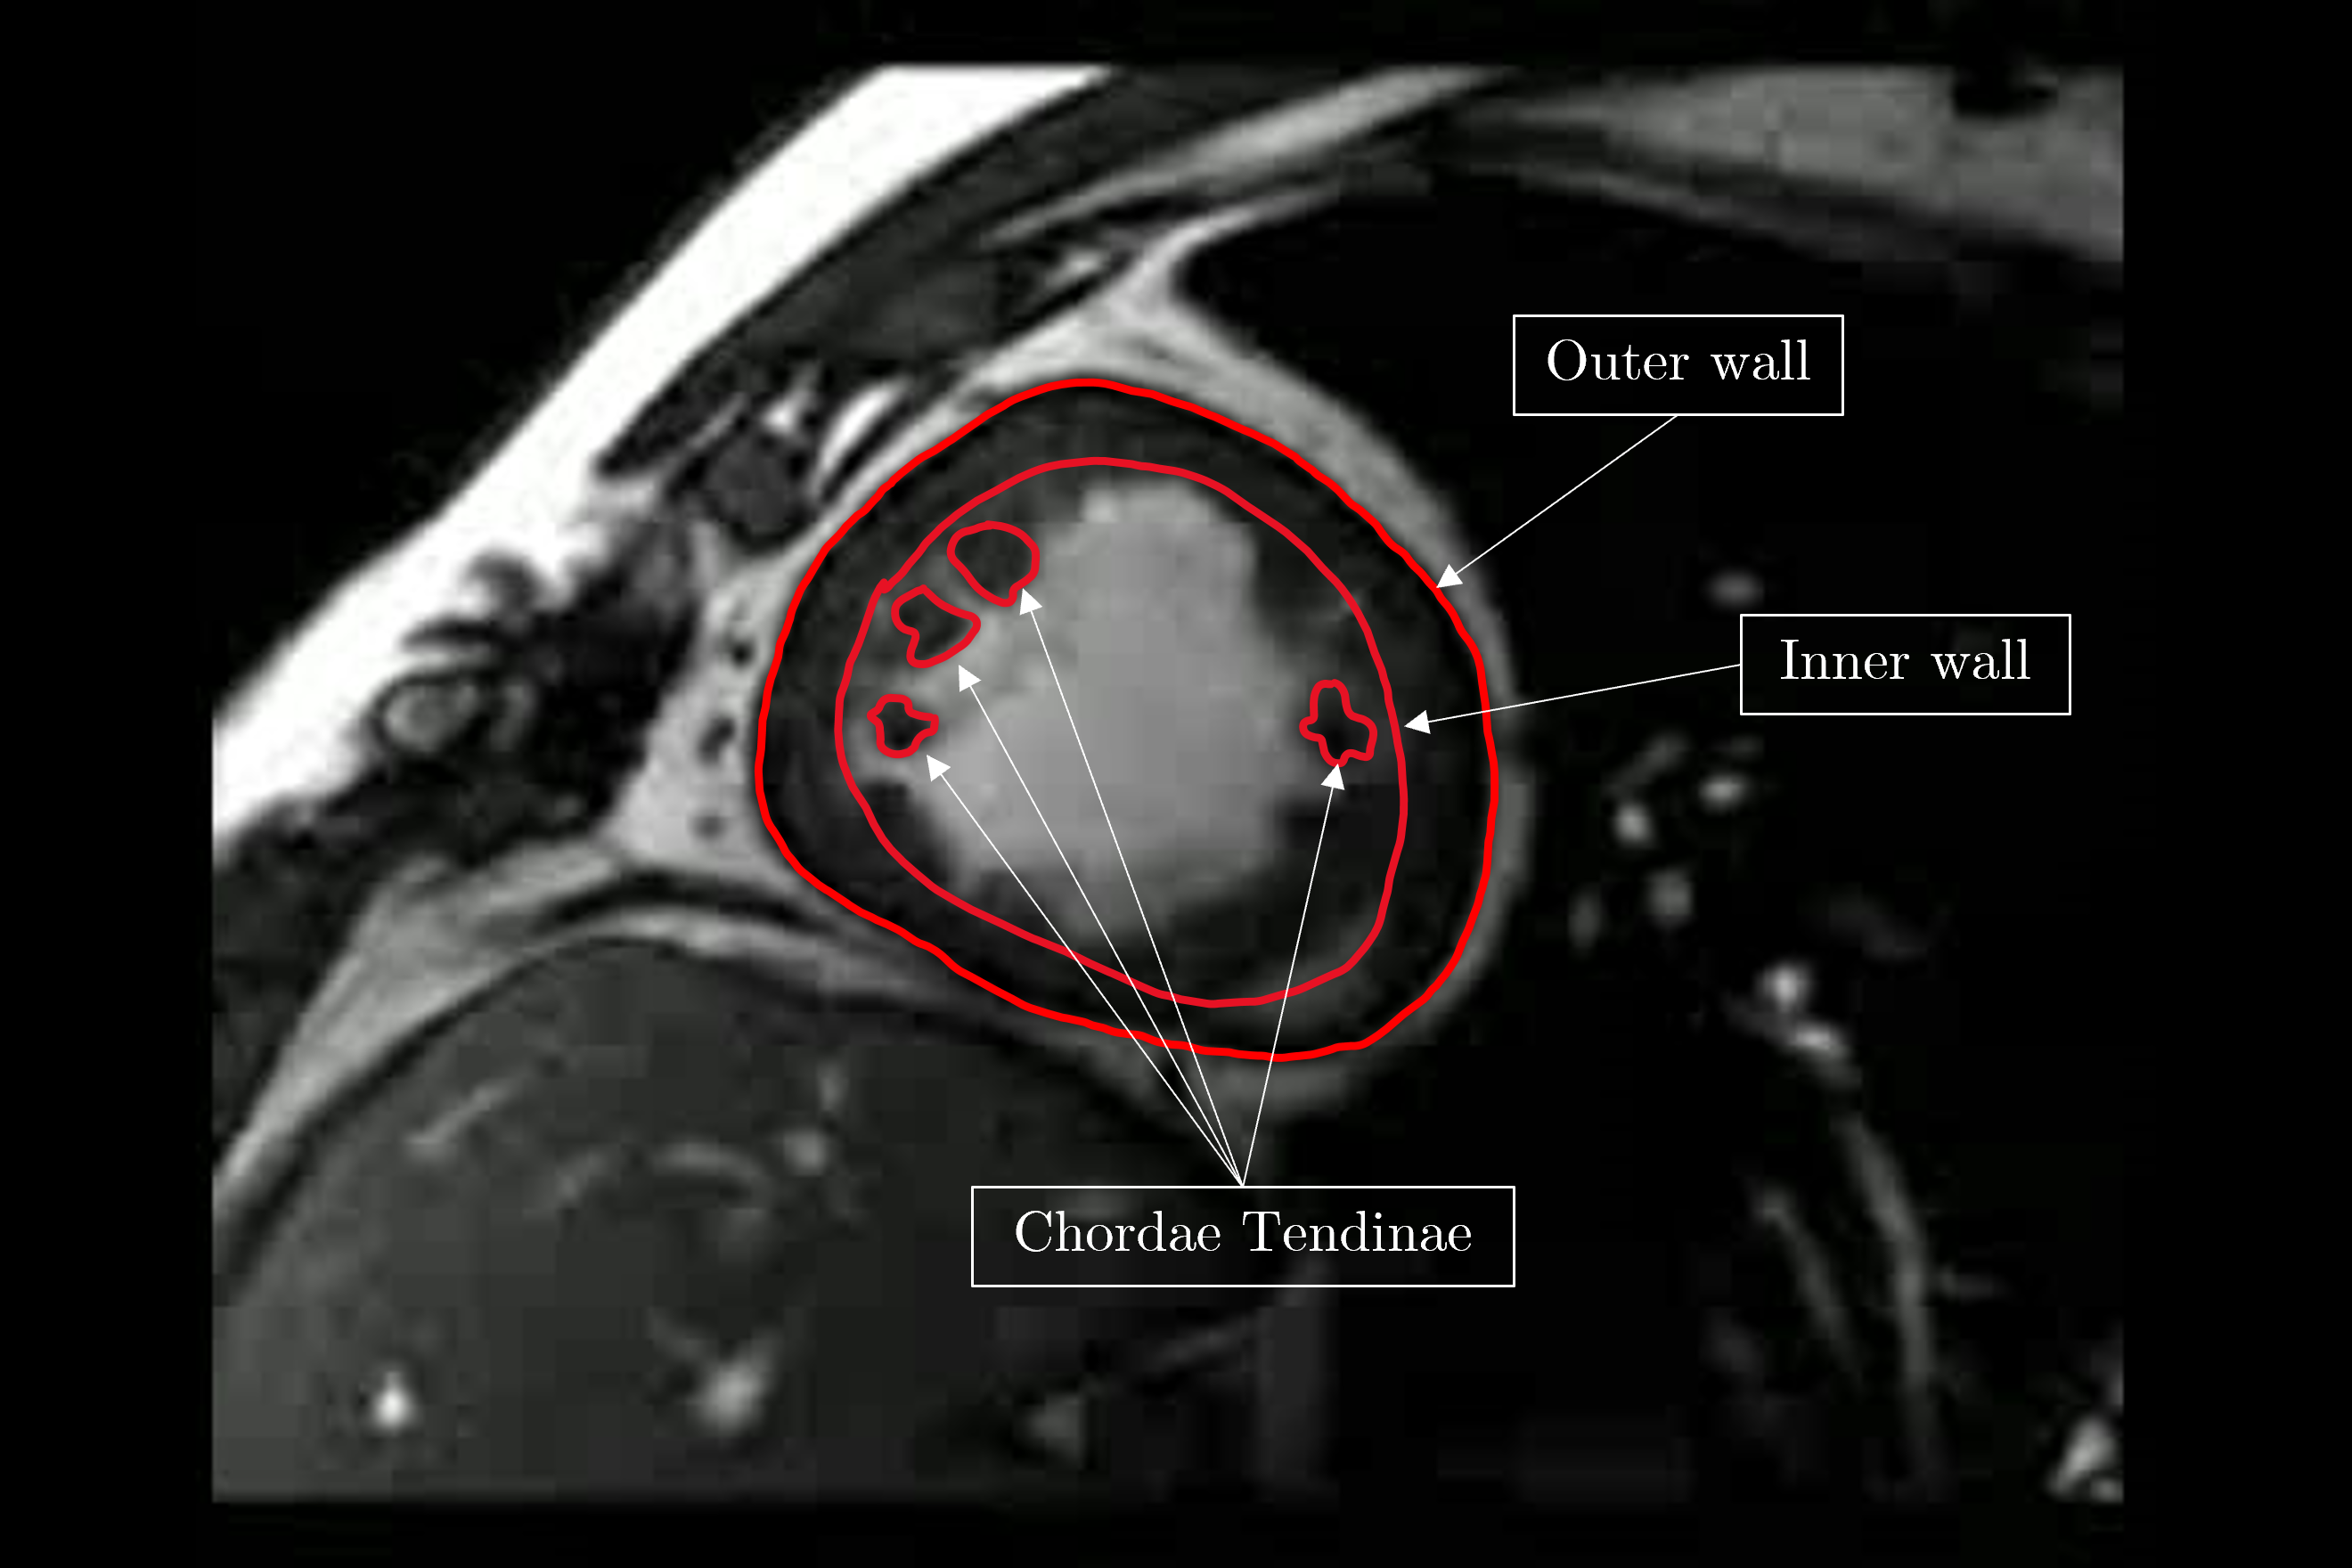
\includegraphics[width=0.8\textwidth]{images/q1_cardiac_anatomy.png}
  \caption{First frame annotated with: left ventricle outer/inner walls, four chordae tendinae.}
  \label{fig:cardiac_anatomy}
\end{figure}

The task is to segment the inner and outer ventricle walls from the rest of the image. The chordae tendinae, commonly known as ``heart strings'', are not part of the inner wall but are fibrous connections that prevent the backflow of blood in the heart \cite{gunnal_2015}. Their proximity to the inner wall presents one of several forseeable challenges. Four chordae tendinae are demarcated in Figure \ref{fig:cardiac_anatomy}, but others are visible; in the bottom right of the ventricle, it is unclear whether the thick band is part of the wall or not. The segmentation task is sufficiently difficult for a human non-medical-expert (the author), and much more so for an automated algorithm!

\newpage
\section{Methodology}

\subsection{Morphology and Contours}

This section describes the approach taken to segment the provided sequence of images using only morphology and contours. The inner and outer walls are treated separately, and both are split into the separate tasks of image segmentation and contour identification.

Before any processing, each frame is cropped to the region surrounding the left ventricle to reduce the likelihood of noise and spurious features impeding segmentation. Figure \ref{fig:frame_cropping} presents the cropped region of the first frame; all other frames are cropped in exactly the same manner.

\begin{figure}[ht]
  \centering
  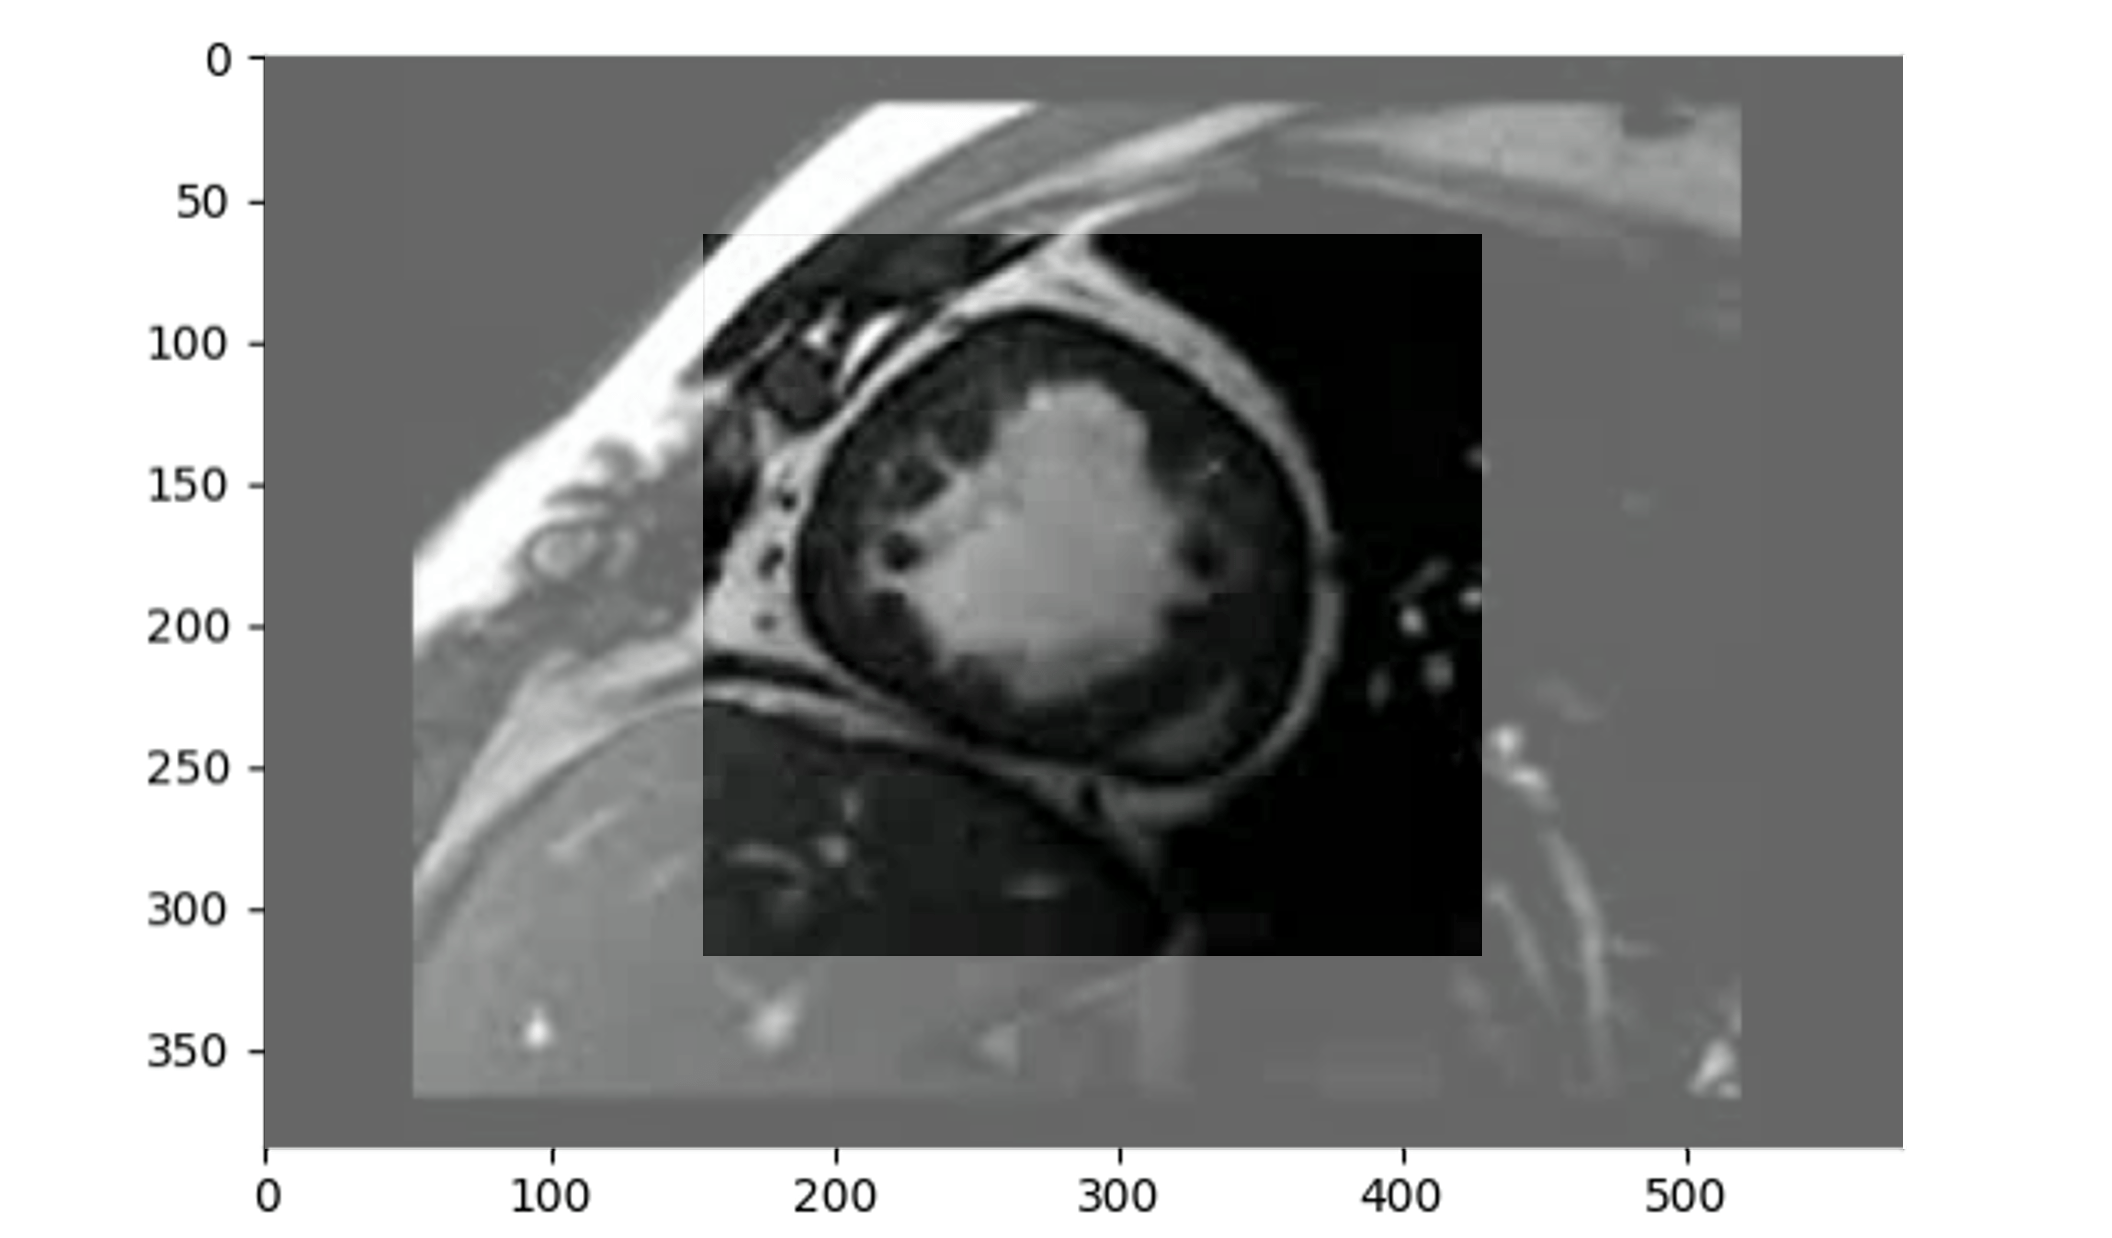
\includegraphics[width=0.6\textwidth]{images/q1_frame_cropping.png}
  \caption{Cropped region of the first frame.}
  \label{fig:frame_cropping}
\end{figure}

The outer wall is addressed first, and represents the more difficult of the inner and outer walls:

\begin{enumerate}
  \item The frame is converted from three-channel grayscale to a single channel.

  \item The frame is binarized using a Gaussian adaptive threshold, with an experimentally-tuned neighbourhood size of 71 pixels, and threshold constant of 10 (which is subtracted from the weighted mean).

  \item Border-connected white regions are cleared, and contours with an area less than an experimentally-tuned threshold of 4000 pixels are filled in with the surrounding colour to remove them. The following steps diverge based on the outcome of this step.

  \item If the frame is non-empty, then the segmented result is returned. Else, if the frame is empty, then the previous step removed all features of the image. In this case, the procedure continues from Step 2, starting with Step 5.

  \item The contours in the frame are sorted and the largest contour is filled with white.

  \item The frame is morphologically opened using a large circular kernel of diameter 11 pixels.

  \item Contours with an area less than 4000 pixels, which were isolated by the morphological opening, are filled in with the surrounding colour to remove them.

\end{enumerate}

The predominant strategy for the segmentation of the outer wall is in Steps 1 to 4. This succeeds when the thresholding separates the ventricle from the cropped frame border and forms a coherent torus-like region. However, in a few frames, the outer wall is difficult to distinguish from the surrounding space, and in these frames the ventricle is connected to the frame border in the thresholded result. As a result, the entire ventricle is cleared as a border-connected region. To address this, Steps 5 to 7 provide an alternative segmentation approach.

The alternative strategy involves forming the entire ventricle into a solid white region then applying a large morphological opening to erase noisy details. The former is done by filling the largest contour with white, which is assumed to be the area inside the ventricle. While this happens to be true for all frames failing the predominant strategy, it is not true for all frames in the sequence. This is a caveat of the method.

Following the segmentation of the outer wall, contour identification is relatively simple:

\begin{enumerate}
  \item The contours in the frame are sorted by area and the largest contour is selected.

  \item The convex hull of the largest contour is taken as the outer ventricle wall.

\end{enumerate}

By design, the ventricle area within the outer wall is the largest remaining contour in the segmented frame, making it easy to identify. The convex hull is returned rather than the contour itself based on the knowledge that the ventricle wall has a smooth convex shape, and concavities are likely the result of noise.

The procedure for the inner wall is considerably simpler. In particular, the segmentation task is much less involved than for the outer wall:

\begin{enumerate}
  \item The frame is converted from three-channel grayscale to a single channel.

  \item The frame is binarized using an experimentally-tuned threshold of 70.

\end{enumerate}

This procedure successfully segments the inner area in all frames, though the chordae tendinae remain as dark regions within or attached to the inner ventricle wall. This is handled by taking the convex hull of the identified contour:

\begin{enumerate}
  \item The contours in the frame are found using the Suzuki and Abe \cite{suzuki_1985} algorithm, enabled by the OpenCV \texttt{findContours} function \cite{opencv_2023a}.

  \item The contours are filtered by extent (ratio of contour to bounding rectangle area \cite{opencv_2023b}), and contours with an extent less than an experimentally-tuned threshold of 0.4 are discarded.

  \item The contours are sorted by area and the largest contour is identified.

  \item The convex hull of the largest contour is taken as the inner ventricle wall.

\end{enumerate}

The approach assumes the inner wall contour is the largest contour by area with an extent greater than 0.4. This assumption holds for all frames, even before cropping, except the last four, in which the left ventricle is contracted and another orifice opens at the bottom of the frame. However, the chance of this spurious identification is eliminated by the cropping.

\newpage
\subsection{Viterbi Algorithm}

This section describes a more complex approach to segmentation, using the Viterbi algorithm. However, compared to the technique presented by Bamford and Lovell \cite{bamford_1998}, out of interest this report presents a different application of the Viterbi algorithm to the segmentation problem. Rather than observing the spatial relationship between points around the trellis, the presented method observes the temporal relationship between the set of points at each angle (i.e. the states are the rows of the trellis rather than the columns).

Before any processing, each frame is cropped in an identical manner to the previous method. Furthermore, the segmentation of both the outer and inner walls also proceed almost identically. The sole difference is that the segmentation of the inner wall applies the same Gaussian adaptive threshold as that of the outer wall for the previous method, rather than a simple threshold.

For brevity, the segmentation steps will not be re-listed. Rather, the application of the Viterbi algorithm will follow on from the segmentation steps presented for the previous approach. The inner and outer walls apply the same steps for Viterbi-based contour identification:

\begin{enumerate}
  \item The states are extracted from the segmented frame, where each state is a distance from the origin to the outer/inner wall along lines defined at regular angular intervals.

  \item For each angle, the Viterbi algorithm is performed on the set of observations representing the distance of the outer/inner wall from the origin over time; the algorithm returns the most likely sequence of distances given the observations.

  \item The sequences of distances for each angle are reconstructed into an outer/inner wall contour for each frame.

  \item The convex hull of the constructed contour is taken as the outer/inner ventricle wall.

\end{enumerate}

Figure \ref{fig:viterbi_obs} presents an example of a set of observations used to inform the Viterbi algorithm.

\begin{figure}[ht]
  \centering
  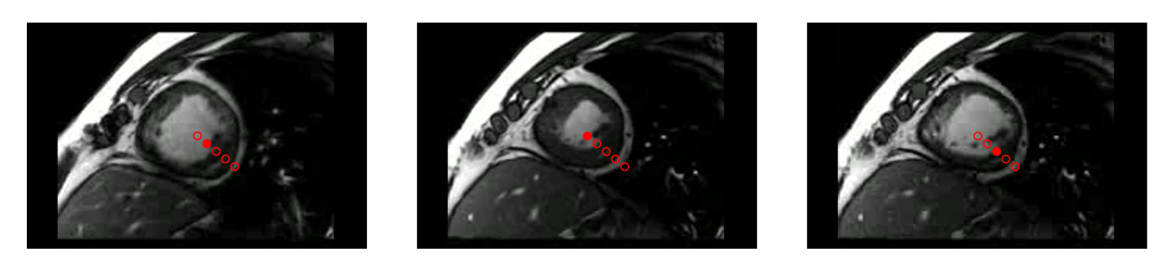
\includegraphics[width=0.9\textwidth]{images/q1_viterbi_obs.png}
  \caption{Highly simplified example of three non-consecutive observations of the inner wall.}
  \label{fig:viterbi_obs}
\end{figure}

Furthermore, the Viterbi algorithm requires the definition of initial, transition, and emittance probabilities. Due to the construction of the problem, the same sets of probabilities apply to every application of the Viterbi algorithm at each angle around the trellis.

The initial states are entirely random, depending on factors such as the trellis origin and the state of the ventricle in an arbitrarily chosen first frame of a sequence. Therefore, a uniform distribution represents the initial state probabilities.

For the transition probabilities, a zero-centred Gaussian distribution with unity standard deviation is used. This reflects the continuous nature of the ventricle wall motion in reality, meaning the probability of transitioning to nearby states is much higher than to those farther away.

For the emittance probabilities, a zero-centred Gaussian distribution with five standard deviation is used. This reflects the fact that an observation is likely to be made close to the actual state, but is more lenient than the transition probabilities due to the known presence of noise.

\newpage
\section{Results}

Figure \ref{fig:ventricle_area} presents the ventricle area over time as determined by both approaches. Note that this result depends only on the segmentation of the inner wall; the efficacy of the outer wall segmentation (the harder task) is inconsequential here.

\begin{figure}[ht]
  \centering
  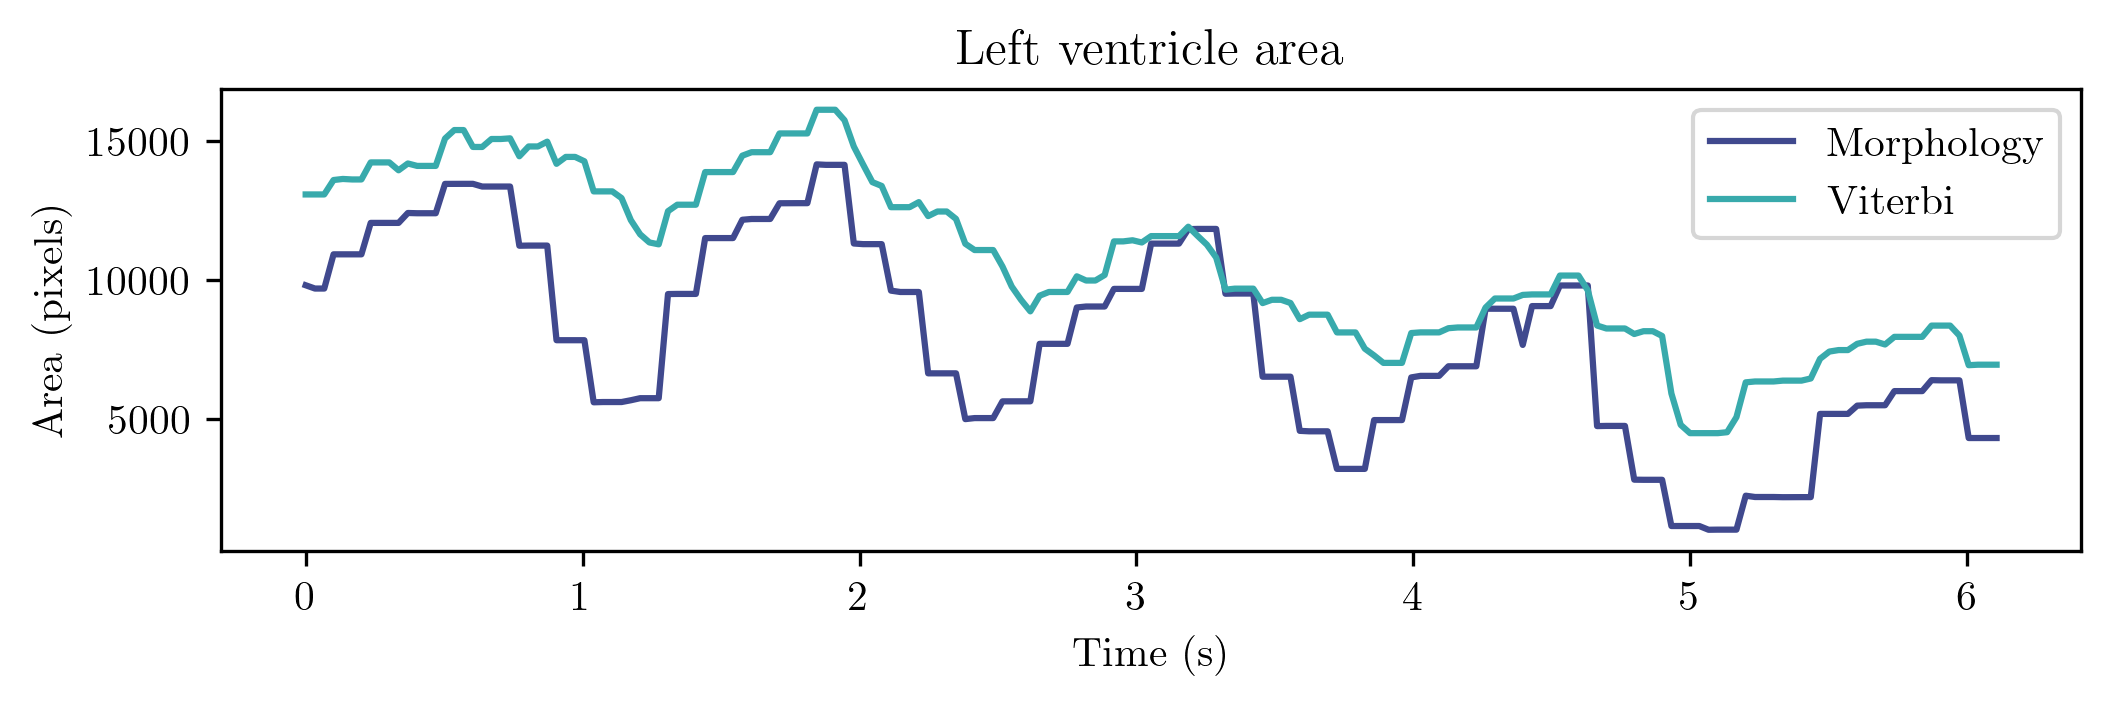
\includegraphics[width=\textwidth]{images/q1_ventricle_area.png}
  \caption{Ventricle area over time as determined using two approaches.}
  \label{fig:ventricle_area}
\end{figure}

The significant observations are that the results follow the same pattern, but the Viterbi approach consistently finds a larger area and has smaller variation between peaks and troughs.

A sample of annotated frames by both approaches is presented in Figure \ref{fig:annotated_frames}.

\begin{figure}[ht]
  \centering
  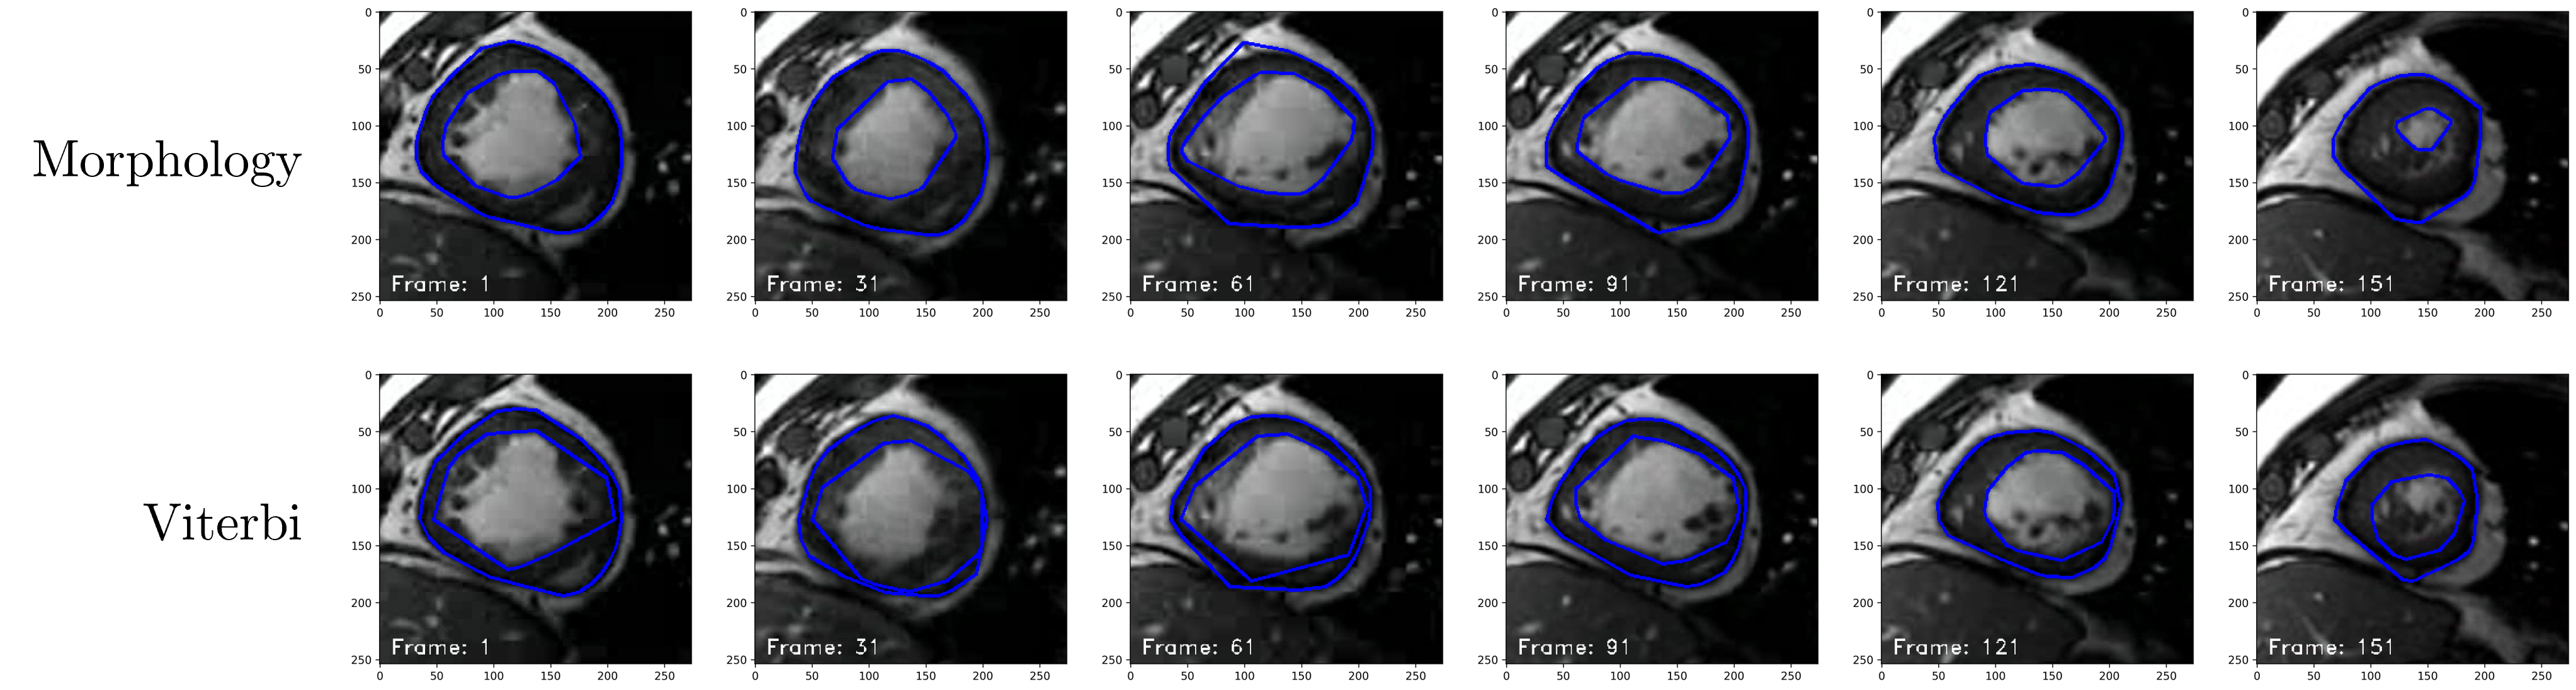
\includegraphics[width=\textwidth]{images/q1_annotated_frames.png}
  \caption{Sample of annotated frames by both approaches, demonstrating plausible results.}
  \label{fig:annotated_frames}
\end{figure}

\newpage
\section{Discussion}

This report has presented two approaches for segmenting the inner and outer walls of a left ventricle in a sequence of cardiac MRI images. The first approach, relying solely on morphology and contouring, is fast and intuitive but non-robust against inadequately thresholded frames. The second approach, based on the Viterbi algorithm, trades runtime speed for better robustness. Figure \ref{fig:ventricle_area} presents the results of both approaches in segmenting the inner ventricle wall, using the area within the identified wall as a proxy. The results of both approaches exhibit a similar pattern, but there are key differences to observe.

Firstly, the Viterbi approach consistently finds a larger area than the morphology approach. This is the result of the approaches applying different methods to segment the inner wall. The morphology approach applies a simple threshold, whereas the Viterbi approach applies a Gaussian adaptive threshold; the latter generally produces a better segmentation between contrasting regions of varying local intensity, and is therefore expected to be more accurate. However, use of the adaptive method for the morphology approach resulted in numerous difficulties stemming from broken regions. Figure \ref{fig:thresh_comparison} presents the thresholded first frame by both approaches, in which the area within the ventricle is clearly larger for the Viterbi approach.

\begin{figure}[ht]
  \centering
  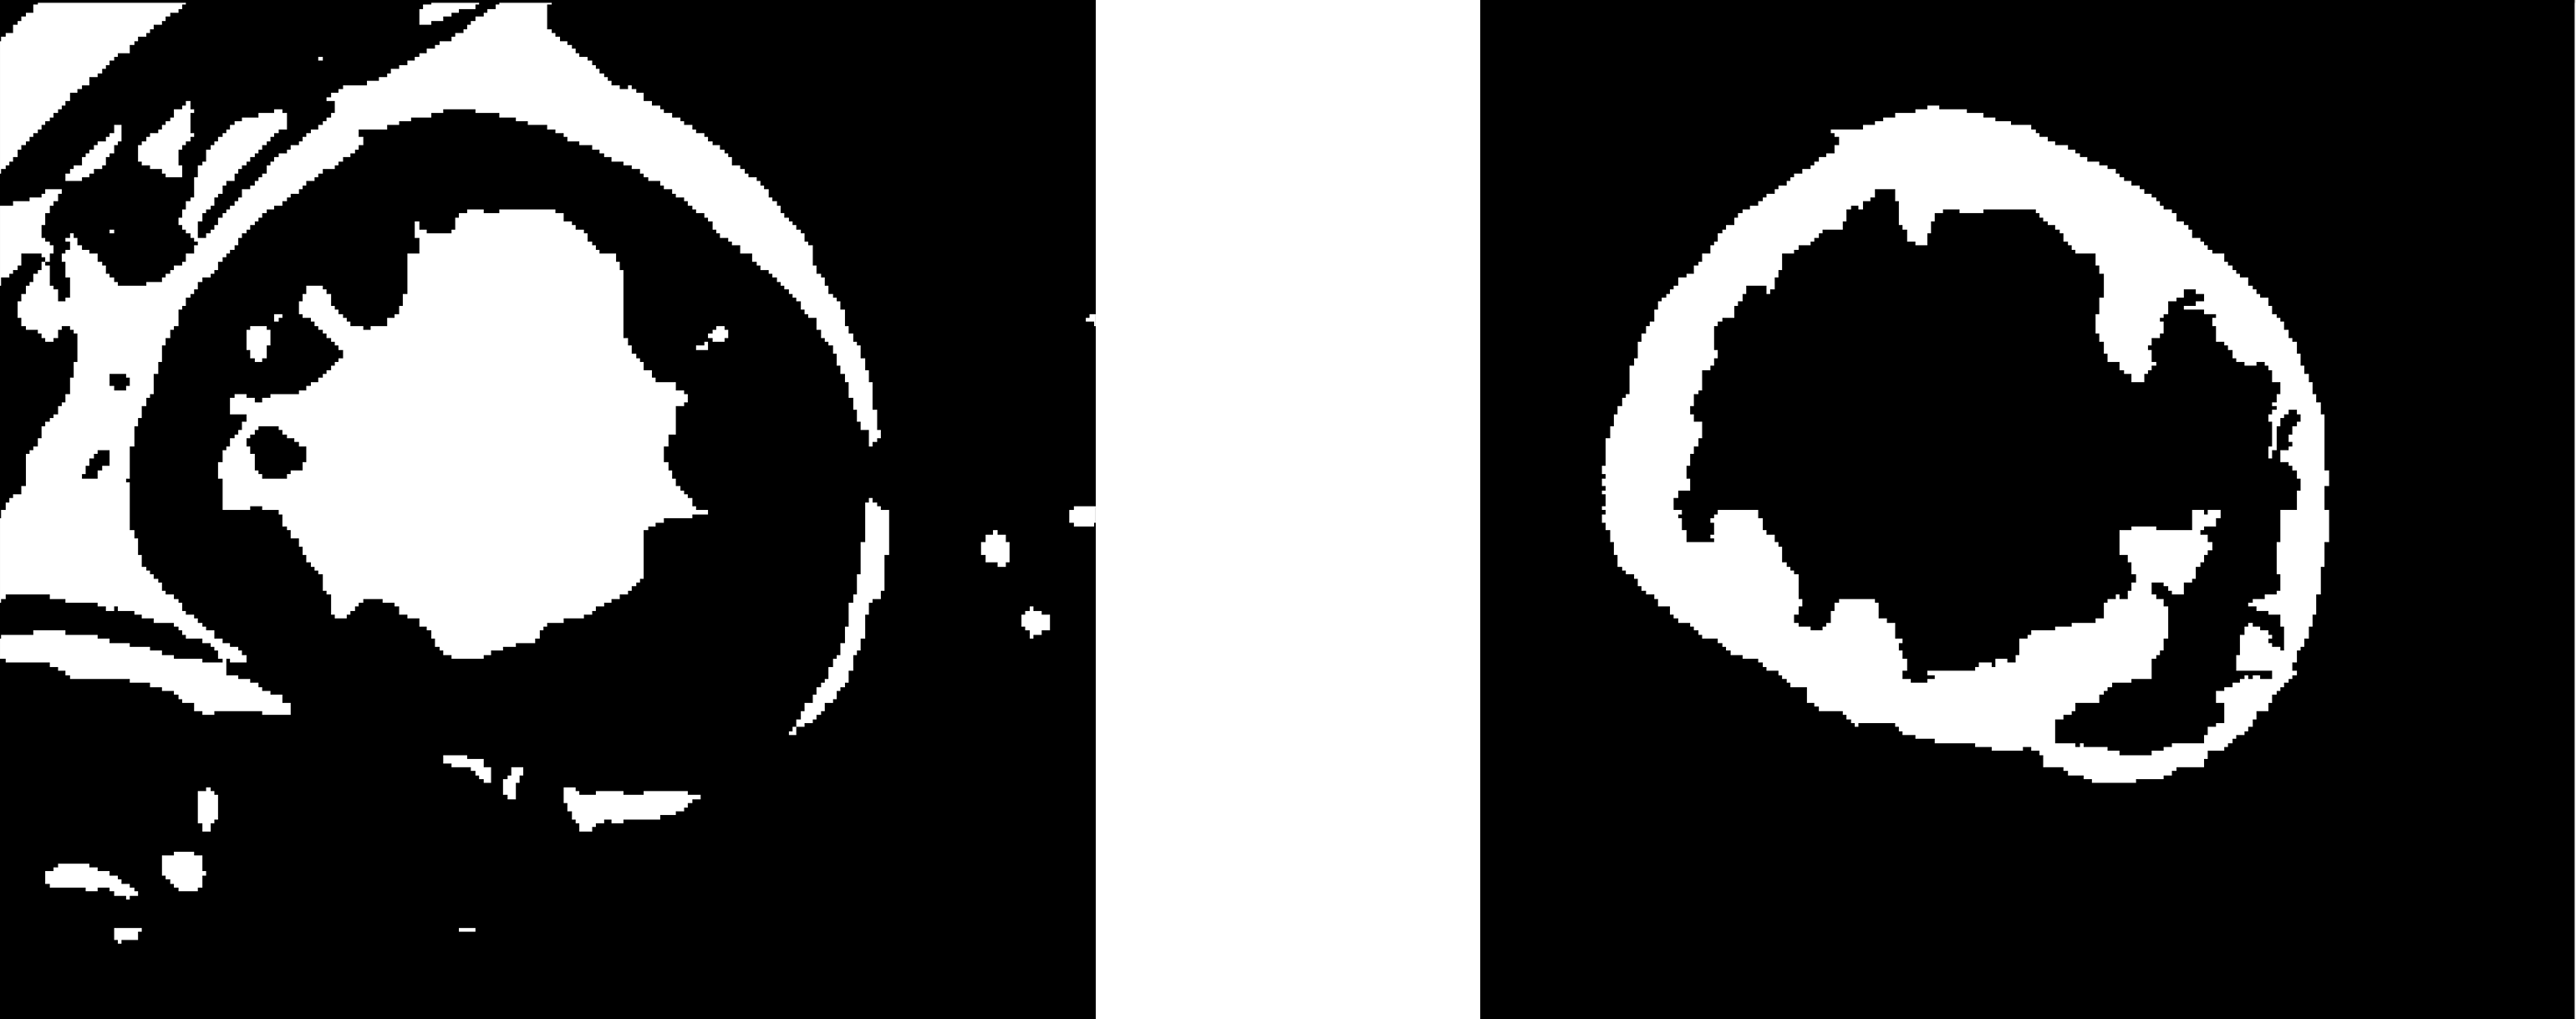
\includegraphics[width=0.6\textwidth]{images/q1_thresh_comparison.png}
  \caption{Thresholded first frame of morphology (left) and Viterbi (right) approaches, demonstrating larger internal area for the Viterbi approach. Note the colours on the left are inverted.}
  \label{fig:thresh_comparison}
\end{figure}

Secondly, the Viterbi approach exhibits smaller variation between peaks and troughs than the morphology approach. This is due to the temporal application of the Viterbi algorithm, as opposed to the spatial application suggested by Bamford and Lovell \cite{bamford_1998}. In the Viterbi algorithm, the transition probability matrix specifies the probability of transitioning from one state to another between successive frames. A Gaussian probability is chosen to represent this, because the continuous motion of the ventricle wall in reality means the probability of a transition from one state to another descreases with the distance between the two states. While a reasonable effort was dedicated to defining an appropriate transition probability model, it is likely that the transition matrix enforces too low a probability on the transition between distant states for the particular frame rate of the image sequence. As a result, the Viterbi algorithm infers a dampened motion of the ventricle wall. This is confirmed by collating contour-annotated frames into a video, and observing that the inner wall contour does not keep up with the true motion of the wall. Brief attempts to improve the transition probability model were met with difficulties manifesting in unexpected contour shapes in certain frames. In this regard, the variation in the area described by the morphology approach is more accurate.

In general, the difficulties associated with processing sequences of images arise from the need to design an algorithm robust enough to correctly handle all frames. This was a difficulty for both the morphology and Viterbi approaches, which both rely on an effective segmentation step to enable contour detection or construction, respectively. The segmentation requires extensive tuning to maximise success on the provided images, and as a result is unlikely to generalise well. The morphology approach is particularly dependant, and frequently fails if the segmentation is not near-perfect. The Viterbi approach is more resilient in this regard, being able to infer a probable state where information is infrequently missing.

Both approaches leave significant room for improvement. For the morphology approach, the segmentation step should be improved to better represent the ventricle wall. This will likely require extensive experimentation to determine a method and parameters that successfully segment all frames. For the Viterbi approach, the transition probabilities require tuning such that the inferred position of the wall does not lag the true position. Also possible would be to combine the methods, such that the Viterbi algorithm is applied to infer missing parts of the segmented ventricle wall only where the morphology approach fails. This could represent a reasonable compromise between speed and robustness.

\section{Conclusion}

In summary, this report presents two relatively simple methods of segmenting the inner and outer walls of a left ventricle in a sequence of cardiac MRI images: a pure morphology and contouring approach, and a Viterbi algorithm approach. Both solutions produce plausible results, but the morphology approach trades some robustness for significantly lower computational complexity, and vice versa for the Viterbi approach. The report concludes with a discussion on the challenges of processing image sequences, and possible improvements to the presented solutions.
